\documentclass[11pt]{article}
\usepackage[a4paper,margin=2.6cm]{geometry}
\usepackage[T1]{fontenc}
\usepackage{lmodern}
\usepackage{microtype}
\usepackage{amsmath,amssymb,amsthm,mathtools}
\usepackage{booktabs,tabularx,array}
\usepackage{enumitem}
\usepackage{xcolor}
\usepackage{tikz}
\usetikzlibrary{arrows.meta,positioning,calc,decorations.pathmorphing}
\usepackage[most]{tcolorbox}
\usepackage[colorlinks=true,linkcolor=blue!50!black,citecolor=blue!50!black,urlcolor=blue!50!black]{hyperref}

\newcommand{\R}{\mathbb{R}}
\newcommand{\T}{\mathbb{T}}
\newcommand{\dd}{\,\mathrm{d}}
\newcommand{\Res}{\mathcal{R}}
\newcommand{\avg}[1]{\langle #1\rangle}
\DeclareMathOperator{\curl}{curl}
\DeclareMathOperator{\supp}{supp}

\theoremstyle{plain}
\newtheorem{theorem}{Theorem}
\newtheorem{proposition}[theorem]{Proposition}
\theoremstyle{remark}
\newtheorem{remark}{Remark}
\newtheorem*{example}{Worked example}

% Provenance tags
\newcommand{\paper}{\textsf{\small[Paper]}}
\newcommand{\chk}{\textsf{\small[Check]}}
\newcommand{\heur}{\textsf{\small[Heuristic]}}
\newcommand{\ctx}{\textsf{\small[Context]}}

\newtcolorbox{keybox}[1]{colback=blue!3,colframe=blue!40!black,fonttitle=\bfseries,title=#1,boxrule=0.6pt,arc=2pt}
\newtcolorbox{statusbox}[1]{colback=orange!4,colframe=orange!60!black,fonttitle=\bfseries,title=#1,boxrule=0.6pt,arc=2pt}

\title{\textbf{How a Forced Navier--Stokes Flow Blows Up}\\[4pt]
\large A guided exposition of OpenAI's finite-time blowup construction\\
for the three-dimensional Navier--Stokes equations\\[2pt]
\normalsize (The Justin Sun Prize problem JSP-000005)}
\author{Thanh Van Nguyen\thanks{Independent. Version~1.0. This exposition was prepared with the assistance of an AI system (Claude, Anthropic); every statement attributed to the source paper was checked against the pinned PDF and repository cited below. Corrections are welcome.}}
\date{29 October 2026}

\begin{document}
\maketitle

\begin{abstract}
In September 2026 OpenAI released a 166-page preprint, \emph{Finite time blowup for Navier--Stokes}~\cite{OAI}, together with a Lean~4 formalization~\cite{OAILean}. For every viscosity $\nu>0$ it constructs a smooth, compactly supported force and a velocity field that starts from rest, keeps bounded kinetic energy, and becomes unbounded at time $t=1$. This addresses the \emph{forced} breakdown alternatives (C) on $\R^3$ and (D) on $\R^3/\mathbb Z^3$ of the Clay Millennium Problem~\cite{Fef}. It does not address the unforced alternatives (A) and (B).

This note explains the construction for a reader who knows basic PDE and fluid mechanics but has not read the paper. We explain why the problem reduces to a cancellation problem for the \emph{momentum residual}. We describe the anisotropic collapsing vortex at the heart of the flow, and how amplified oscillatory pulses supply exactly the momentum flux that the vortex lacks. We then show how an infinite correction cycle makes the residual vanish to every order at the singular point, and how localization, a Borel-type extension and a uniqueness argument finish the proof. We also describe what the Lean development certifies. Along the way we give self-contained scale checks and two toy models: plane-wave Reynolds stress and centrifugal amplification. Every statement is tagged so the reader can see which claims come from the paper, which we verified by hand, and which are heuristics.
\end{abstract}

\begin{statusbox}{Status of the result (as of 29 October 2026)}
\begin{itemize}[leftmargin=1.2em,itemsep=1pt]
\item \textbf{Claimed:} Theorem~1.1 of~\cite{OAI}, establishing alternatives (C) and (D) in Fefferman's statement~\cite{Fef}, for every $\nu>0$.
\item \textbf{Machine-checked (as reported):} Lean statements of (C) and (D) are proved in the repository~\cite{OAILean} at commit \texttt{f9e8bc5b}. The Comparator challenge permits only the axioms \texttt{propext}, \texttt{Quot.sound} and \texttt{Classical.choice} (\S\ref{sec:lean}). \emph{The author of this note did not rebuild the project.}
\item \textbf{Not yet established:} independent peer review. The Justin Sun Prize catalog records the problem as Solved, with independent review pending. The MathDB page lists the claim as unverified. The Clay Institute lists the problem as active.
\item \textbf{Not claimed by anyone:} alternatives (A) and (B), the \emph{unforced} global regularity or breakdown questions. These remain open.
\end{itemize}
\end{statusbox}

\paragraph{Reading conventions.} \paper{} marks a statement taken from~\cite{OAI} and gives its location there. \chk{} marks a short computation we carried out ourselves to confirm a stated scaling. \heur{} marks a simplified model chosen to convey a mechanism; it is not the paper's argument. \ctx{} marks background from the wider literature.

\tableofcontents

%======================================================================
\section{The question and the answer}
%======================================================================

\subsection{The Clay formulation}
Fefferman's official statement~\cite{Fef} concerns the incompressible Navier--Stokes equations in three dimensions,
\begin{equation}\label{eq:NS}
\partial_t u + (u\cdot\nabla)u = \nu\Delta u - \nabla p + f,\qquad \nabla\cdot u = 0,\qquad u(x,0)=u^\circ(x).
\end{equation}
It offers four alternatives, and a proof of any one of them resolves the problem:
\begin{itemize}[itemsep=1pt]
\item[(A)] global smooth bounded-energy solutions on $\R^3$ for all smooth, rapidly decaying, divergence-free data, with $f\equiv 0$;
\item[(B)] the same on the torus $\R^3/\mathbb Z^3$;
\item[(C)] \emph{breakdown on $\R^3$}: there exist smooth, rapidly decaying $u^\circ$ and $f$ (with $|\partial_x^\alpha\partial_t^m f|\le C_{\alpha mK}(1+|x|+t)^{-K}$) such that no solution $(u,p)$ is smooth on $\R^3\times[0,\infty)$ and has bounded energy $\sup_t\int|u|^2\,dx<\infty$;
\item[(D)] \emph{breakdown on the torus}: the periodic analogue of (C), with forces decaying in time.
\end{itemize}
Alternatives (C) and (D) \emph{allow an external force}. This is the opening the construction uses.

\subsection{The theorem}
\begin{theorem}[\paper{} Theorem~1.1]\label{thm:main}
For every $\nu>0$ there exist a force $f\in C_c^\infty(\R^3\times(0,\infty);\R^3)$, a compact set $K\subset\R^3$, and smooth velocity and pressure fields $u,p$ on $\R^3\times[0,1)$ solving \eqref{eq:NS} with $u(\cdot,0)=0$, such that $\supp u(\cdot,t)\cup\supp p(\cdot,t)\subset K$ for $0\le t<1$ and
\[
\sup_{0\le t<1}\|u(t)\|_{L^2(\R^3)}<\infty,\qquad \limsup_{t\uparrow1}\|u(t)\|_{L^\infty(\R^3)}=\infty .
\]
Consequently there is no smooth solution on $\R^3\times[0,\infty)$ with the same force and initial datum whose kinetic energy is uniformly bounded.
\end{theorem}

The zero initial datum is trivially smooth, divergence-free and decaying, and a compactly supported smooth force satisfies every decay bound in~(C). So Theorem~\ref{thm:main} is an instance of~(C). Rescaling and periodizing give~(D) (Corollary~10.6 of~\cite{OAI}; see \S\ref{sec:torus}).

\subsection{What the theorem does \emph{not} say}
\begin{itemize}[itemsep=1pt]
\item It does not show that \emph{unforced} smooth flows can blow up, and it does not prove global regularity. Those are (A) and (B).
\item The force is not a ``natural'' stirring. It is engineered so that it extends smoothly through the singular time. Its role is explained in \S\ref{sec:residual}.
\item The singular flow is smooth before $t=1$ and has bounded energy and finite total dissipation (\S\ref{sec:energy}). So the result says something about smooth solutions, not about weak solutions.
\end{itemize}

%======================================================================
\section{Background: why three dimensions are hard}\label{sec:background}
%======================================================================

\subsection{Scaling and supercriticality}
\ctx{} If $(u,p,f)$ solves \eqref{eq:NS} with viscosity $\nu$, then
$u_\lambda(x,t)=\lambda u(\lambda x,\lambda^2t)$, $p_\lambda=\lambda^2p(\lambda x,\lambda^2 t)$ and $f_\lambda=\lambda^3 f(\lambda x,\lambda^2t)$ solve it with the same $\nu$.
\chk{} The energy transforms as $\|u_\lambda(t)\|_{L^2}^2=\lambda^{2}\lambda^{-3}\|u(\lambda^2t)\|_{L^2}^2=\lambda^{-1}\|u\|_{L^2}^2$. Zooming into small scales ($\lambda\to\infty$) therefore makes the energy bound \emph{weaker}. This is the precise sense in which the energy identity is \emph{supercritical}: it cannot by itself rule out concentration at small scales. Scale-invariant quantities such as $\|u\|_{L^3}$ or $\sqrt{T-t}\,\|u(t)\|_{L^\infty}$ are \emph{critical}.

A smooth solution can be continued as long as $\|u(t)\|_{L^\infty}$ stays bounded. So (A) and (B) are equivalent to ruling out finite-time blowup. Leray~\cite{Leray} showed that if blowup happens at time $T$ for the unforced problem, then $\|u(t)\|_{L^\infty}\gtrsim (\nu/(T-t))^{1/2}$.

\subsection{What was known}
\ctx{} \paper{} (\S1.1 of~\cite{OAI}):
\begin{itemize}[itemsep=1pt]
\item \emph{Leray (1934)} built global finite-energy weak solutions~\cite{Leray}. \emph{Caffarelli--Kohn--Nirenberg} showed that the singular set of a suitable weak solution has zero one-dimensional parabolic Hausdorff measure~\cite{CKN}. \emph{Escauriaza--Seregin--\v{S}ver\'ak} proved regularity for the unforced problem under an $L^\infty_tL^3_x$ bound~\cite{ESS}.
\item \emph{Ne\v{c}as--R\r{u}\v{z}i\v{c}ka--\v{S}ver\'ak} and \emph{Tsai} ruled out Leray's backward self-similar blowup ansatz $u=(T-t)^{-1/2}U(x/\sqrt{T-t})$ in natural classes~\cite{NRS,Tsai}. So any unforced blowup must be more complicated than exact self-similarity.
\item \emph{Tao (2016)} proved blowup for an \emph{averaged} Navier--Stokes equation that keeps the energy cancellation of the nonlinearity~\cite{Tao}. This showed that energy methods alone cannot settle the problem.
\item \emph{Buckmaster--Vicol} and \emph{Albritton--Brué--Colombo} proved non-uniqueness of weak and Leray--Hopf solutions, the latter with a force~\cite{BV,ABC}. \emph{Córdoba--Martínez-Zoroa} constructed forced singularities for 3D Euler, and \emph{Córdoba--Martínez-Zoroa--Zheng} extended this to hypodissipative Navier--Stokes~\cite{CMZ,CMZZ}. These constructions use successive amplification across scales.
\end{itemize}
The new construction follows the forced-amplification line, but at full viscosity, with a smooth force and with true (not averaged) nonlinearity. In the words of the paper, ``oscillatory pulses generate a mean momentum flux that supplies the missing force on a collapsing background vortex'' (\S1.1).

%======================================================================
\section{The reformulation: choose the flow, read off the force}\label{sec:residual}
%======================================================================

For any smooth divergence-free $u$ and any smooth $p$, define the \emph{momentum residual}
\begin{equation}\label{eq:residual}
\Res(u,p) := \partial_t u + (u\cdot\nabla)u - \nu\Delta u + \nabla p .
\end{equation}
Then $(u,p)$ solves \eqref{eq:NS} with force $f:=\Res(u,p)$, by definition. Every flow is a forced Navier--Stokes flow.

\begin{keybox}{The real problem}
Find $(u,p)$, smooth for $t<1$, with $\|u(t)\|_{L^\infty}\to\infty$ as $t\uparrow1$, such that $\Res(u,p)$ \emph{and all its space-time derivatives} extend continuously through $t=1$. The force must then extend to a smooth, compactly supported function on $\R^3\times(0,\infty)$.
\end{keybox}

Each term of \eqref{eq:residual} blows up separately near the singular point, so their sum has to cancel to infinite order. The paper states this as a flatness estimate \paper{} (eq.~(3.4), Theorem~3.1(iii)):
\begin{equation}\label{eq:flat}
|\partial_x^\alpha\partial_t^b\Res(u,p)|\le C_{\alpha,b,N,X_1}\,q^N\qquad\text{for all }\alpha,b,N,
\end{equation}
where $q\to0$ is a concentration scale that measures distance to the singular point (\S\ref{sec:geometry}). \emph{All the difficulty of the paper lies in achieving \eqref{eq:flat}.}

\begin{remark}[Why a naive vortex fails]
\heur{} Take a smooth vortex profile and collapse it self-similarly. The residual is then the profile's failure to solve the self-similar equations, multiplied by a negative power of $T-t$. Unless the profile solves those equations exactly, the force blows up. The obstructions in~\cite{NRS,Tsai} block exact self-similar solutions in natural classes. The paper avoids them in two ways: it uses \emph{two different contraction rates} (\S\ref{sec:geometry}), and it does not ask the vortex to balance its own momentum. Instead, a second, oscillatory component supplies the missing momentum flux (\S\ref{sec:pulses}).
\end{remark}

%======================================================================
\section{The geometry of the collapsing vortex}\label{sec:geometry}
%======================================================================

\subsection{The physical picture}
\paper{} (\S2.1 of~\cite{OAI}) Use cylindrical coordinates $(r,\theta,z)$ about the vertical axis and write $\tau=1-t$. The leading flow $u^{(0)}$ is axisymmetric. In the central core, fluid \emph{spirals inward} toward the axis and \emph{flows out axially}, up and down on opposite sides of a dividing layer near $z=0$. Pressure decreases toward the axis and supplies the centripetal force.

Spin-up has a simple cause. Without torque, angular momentum per unit mass $ru_\theta$ is conserved, so fluid carried inward rotates faster. Viscosity carries angular momentum back outward, and the characteristic speed grows as the balance between these two effects. Incompressibility forces the incoming fluid to leave along the axis, and this keeps the inflow going.

\begin{figure}[h]
\centering
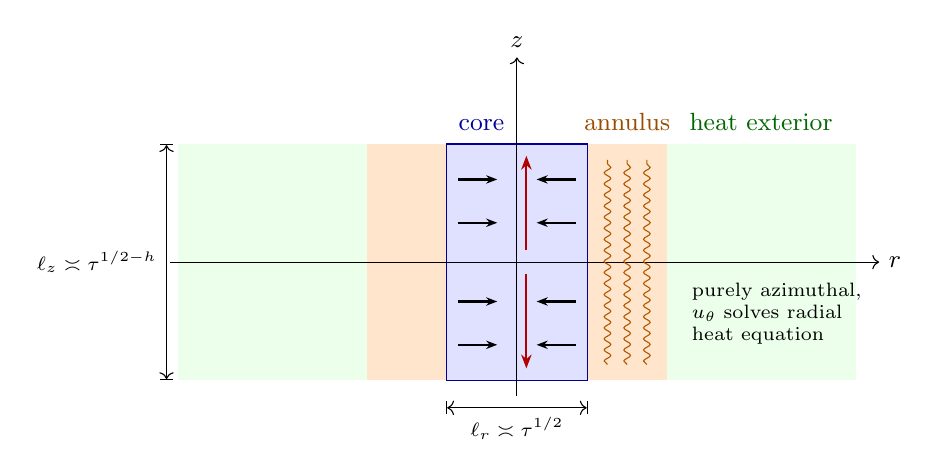
\begin{tikzpicture}[scale=1.0]
 \fill[blue!12] (-0.9,-1.5) rectangle (0.9,1.5);
 \draw[blue!60!black] (-0.9,-1.5) rectangle (0.9,1.5);
 \fill[orange!20] (0.9,-1.5) rectangle (1.9,1.5);
 \fill[orange!20] (-1.9,-1.5) rectangle (-0.9,1.5);
 \fill[green!8] (1.9,-1.5) rectangle (4.3,1.5);
 \fill[green!8] (-4.3,-1.5) rectangle (-1.9,1.5);
 \draw[->] (-4.4,0)--(4.6,0) node[right]{\small $r$};
 \draw[->] (0,-1.7)--(0,2.6) node[above]{\small $z$};
 \node[blue!60!black,anchor=south] at (-0.45,1.55) {\small core};
 \node[orange!60!black,anchor=south] at (1.4,1.55) {\small annulus};
 \node[green!40!black,anchor=south] at (3.1,1.55) {\small heat exterior};
 \foreach \y in {-1.05,-0.5,0.5,1.05}{
   \draw[-{Stealth[length=4pt]},thick] (0.75,\y) -- (0.25,\y);
   \draw[-{Stealth[length=4pt]},thick] (-0.75,\y) -- (-0.25,\y);}
 \draw[-{Stealth[length=5pt]},thick,red!70!black] (0.12,0.15)--(0.12,1.35);
 \draw[-{Stealth[length=5pt]},thick,red!70!black] (0.12,-0.15)--(0.12,-1.35);
 \foreach \x in {1.15,1.4,1.65}{ \draw[orange!70!black,decorate,decoration={snake,amplitude=1.2pt,segment length=4pt}] (\x,-1.3)--(\x,1.3);}
 \node[align=left,font=\scriptsize] at (3.3,-0.65) {purely azimuthal,\\ $u_\theta$ solves radial\\ heat equation};
 \draw[|<->|] (-0.9,-1.85)--(0.9,-1.85) node[midway,below]{\scriptsize $\ell_r\asymp\tau^{1/2}$};
 \draw[|<->|] (-4.45,-1.5)--(-4.45,1.5) node[midway,left]{\scriptsize $\ell_z\asymp\tau^{1/2-h}$};
\end{tikzpicture}
\caption{Schematic radial--axial section at a fixed time (not to scale; after Figures~1--3 of~\cite{OAI}). Black arrows show radial inflow and red arrows axial outflow; the swirl $u_\theta$ points out of the page. The pulses live in the annulus. Both lengths shrink, and the radius shrinks faster than the height.}
\label{fig:geometry}
\end{figure}

\subsection{Scales}
\paper{} (\S2.1, \S3.1) Fix $0<h<1/100$ and set $A=\tfrac12+h$, $D=\tfrac12-h$. Then
\begin{equation}\label{eq:scales}
\ell_r\asymp\tau^{1/2},\qquad \ell_z\asymp\tau^{1/2-h},\qquad |u^{(0)}_\theta|,|u^{(0)}_z|\asymp\tau^{-1/2-h},\qquad |u^{(0)}_r|=O(\tau^{-1/2}).
\end{equation}
The core is an increasingly slender column ($\ell_r/\ell_z\asymp\tau^h\to0$). The swirl vanishes on the axis, and along a fixed similarity radius it grows like $\tau^{-A}$: Theorem~3.1(iv) gives $u_\theta(\sqrt{2X_{\rm in}\tau},0,0,1-\tau)=\tau^{-A}(e_0+O(\tau^{2h}))$ with $e_0>0$.

\begin{table}[h]
\centering\small
\begin{tabular}{@{}lll@{}}
\toprule
Quantity & Scale & Consequence \\
\midrule
Core volume $\ell_r^2\ell_z$ & $\tau^{3/2-h}$ & shrinks to the origin\\
Kinetic energy $\ell_r^2\ell_z|u|^2$ & $\tau^{1/2-3h}\to0$ & energy stays bounded\\
Dissipation rate $\ell_r^2\ell_z|\partial_r u|^2$ & $\tau^{-1/2-3h}$ & integrable in time iff $h<1/6$\\
Swirl Reynolds number $|u_\theta|\ell_r/\nu$ & $\tau^{-h}\to\infty$ & many turns per diffusion time\\
Radial Reynolds number $|u_r|\ell_r/\nu$ & $O(1)$ & viscosity competes with inflow\\
Axial/radial diffusion $\ell_r^2/\ell_z^2$ & $\tau^{2h}\to0$ & small parameter for corrections\\
$\sqrt{\tau}\,\|u\|_{L^\infty}$ & $\tau^{-h}\to\infty$ & faster than the self-similar rate\\
$\|u\|_{L^3(\text{core})}^3$ & $\tau^{-4h}\to\infty$ & critical norm diverges (slowly)\\
\bottomrule
\end{tabular}
\caption{Scales of the leading core flow. The first six rows are stated in~\cite{OAI} (\S2.1, \S3.5). \chk{} We recomputed all rows from \eqref{eq:scales}; the last two are our own consequences of \eqref{eq:scales}.}
\label{tab:scales}
\end{table}

\begin{example}[\chk{} energy and dissipation]
The kinetic energy is $\tau^{3/2-h}\cdot(\tau^{-1/2-h})^2=\tau^{1/2-3h}$. The radial derivative scale is $\tau^{-1/2-h}/\tau^{1/2}=\tau^{-1-h}$, so the dissipation is $\tau^{3/2-h}\cdot\tau^{-2-2h}=\tau^{-1/2-3h}$. This is integrable on $(0,\tau_0)$ exactly when $\tfrac12+3h<1$, that is $h<1/6$. Both match \S3.5 of~\cite{OAI}. The blowup is invisible to the energy, but very visible to the critical quantity $\sqrt\tau\,\|u\|_\infty\asymp\tau^{-h}$. This is consistent with the lower bound of~\cite{Leray}.
\end{example}

\subsection{Why the axial profile is tilted}
\paper{} (\S2.1) The core must also create enough \emph{shear} at its edge to amplify the pulses of \S\ref{sec:pulses}. Away from the mid-plane, axial flow brings in angular momentum from faster-rotating layers, which makes the angular velocity drop steeply with radius. With exact up--down symmetry this effect would vanish at $z=0$, and so would $u_z(r,0,t)$. The authors therefore tilt the axial profile slightly upward, so that the radial shear of $u_z$ supplies amplification near the mid-plane where the rotational mechanism is weak.

\subsection{Similarity coordinates}
\paper{} (\S3.1, eq.~(3.2)) The two contraction rates are resolved by coordinates $(X,\eta,q)$ with
\[
\tau=q(1-\eta^2),\qquad z=q^{D}\eta,\qquad X=\frac{r^2}{2q},\qquad -1<\eta<1 .
\]
The leading fields are then given by profiles $E,U,\Pi$ and a stream-function-type quantity $V_0$:
\[
u_\theta^{(0)}=q^{-A}E(X,\eta),\quad u^{(0)}_z=q^{-A}U(X,\eta),\quad ru^{(0)}_r=V_0,\quad p^{(0)}=q^{-2A}\Pi,
\]
\[
\Pi(X,\eta)=-\!\int_X^\infty\frac{E(x,\eta)^2}{2x}\dd x .
\]
Here $q\asymp\tau+|z|^{1/D}$, so $q\to0$ means approaching the singular point $(x,t)=(0,1)$. The endpoints $\eta=\pm1$ describe $t=1$ away from it. \chk{} At $\eta=0$ we have $q=\tau$, and $X\asymp1$ means $r\asymp\tau^{1/2}$ while $|\eta|\le\eta_c$ means $|z|\lesssim\tau^{1/2-h}$. This recovers \eqref{eq:scales}.

\subsection{The exterior}
\paper{} (\S2.3, Theorem~3.1(iii)) Far out ($X\ge X_{\rm ext}$) the flow is purely azimuthal and height-independent: $u=K(r,\tau)e_\theta$ with $K=r^{-1-2h}H_{\rm ext}(\tau/r^2)$, solving the swirl heat equation $-\partial_\tau K=\partial_r^2K+r^{-1}\partial_rK-r^{-2}K$. Its momentum residual vanishes identically. At each fixed $r>0$ the fields have smooth limits as $\tau\to0$. This is what later allows a spatial cutoff whose force stays smooth through $t=1$.

%======================================================================
\section{The missing force is a stress in an annulus}\label{sec:stress}
%======================================================================

The inner core solves its leading momentum balance, and so does the heat exterior. The problem is the joining region, the \emph{annulus} $X_a<X<X_b$. There the background leaves a residual that blows up as $t\uparrow1$ (\S2.2).

\paragraph{Writing the residual as a divergence.} \paper{} (\S3.2) Let $R^{(0)}_\theta,R^{(0)}_z$ be the tangential momentum residuals of the leading field. The paper writes them as cylindrical divergences of a stress $T=(T_{r\theta},T_{rz})$:
\[
R^{(0)}_\theta=-(\partial_r+2/r)T_{r\theta},\qquad R^{(0)}_z=-(\partial_r+1/r)T_{rz},
\]
\[
T_{r\theta}(r)=-\frac1{r^2}\int_0^r s^2R^{(0)}_\theta(s)\dd s,\qquad T_{rz}(r)=-\frac1r\int_0^r sR^{(0)}_z(s)\dd s .
\]
For $T$ to vanish outside the annulus, the residual must vanish in the core and in the exterior, and two moment identities must hold:
\[
\int_0^\infty r^2R^{(0)}_\theta\dd r=0,\qquad \int_0^\infty rR^{(0)}_z\dd r=0 .
\]
\heur{} Physically, the annulus does not need a net injection of angular or axial momentum. It needs momentum to be \emph{moved radially}, and a radial flux of momentum is exactly what a stress describes. Section~\ref{sec:pulses} shows that a velocity field can supply such a stress through its own nonlinearity.

\paragraph{Matching five radial integrals.} \paper{} (\S3.2, Lemma~4.4) The pressure and the radial velocity depend on cumulative radial integrals. Joining an inner solution to a prescribed exterior requires matching \emph{five} radial integrals (eq.~(4.15)). These govern the pressure, the radial velocity and the stress. Matching them is the content of Appendices~A and~B (axis problem solved analytically in Proposition~B.2, joining in Corollary~B.10, moment correction in Proposition~B.8).

\paragraph{The admissible stress cone.} Section~\ref{sec:pulses} explains that pulses can only produce stresses in an open cone $\{c_1v_1+c_2v_2:c_1,c_2>0\}$, where the directions $v_1,v_2$ are set by the local background. The profile must therefore be chosen so that $T$ lies inside this cone at every point of the annulus. This is the \emph{admissible stress cone condition} (Lemma~4.5).

\paragraph{A logarithmic oscillation.} \paper{} (\S3.2 step~4, Proposition~C.2) To enforce the cone condition, the authors add to the profile a radial oscillation with phase $N\log X$ and amplitude $O(N^{-1})$, with $N$ a large integer. Applying $X\partial_X$ to it gives an \emph{order-one} change in the radial shear, while profile values and radial moments change only by $O(N^{-1})$. The shear then traces a periodic curve that satisfies the cone condition, and a separate localized correction restores the five integrals exactly (Proposition~C.3).

\heur{} This is a standard trick: a small, rapidly oscillating perturbation controls derivatives without disturbing the function. Here it steers the \emph{shear}, which determines the cone, while leaving the \emph{values} that determine the matching conditions almost unchanged.

%======================================================================
\section{Pulses: making the fluid supply its own force}\label{sec:pulses}
%======================================================================

\subsection{The algebraic identity}
\paper{} (\S3.3) For a divergence-free increment $w$ with pressure increment $\pi$,
\begin{equation}\label{eq:increment}
\Res(u_B+w,p_B+\pi)=\Res(u_B,p_B)+L_{u_B}(w,\pi)+\nabla\cdot(w\otimes w),
\end{equation}
where $L_{u_B}(w,\pi)=\partial_tw+(u_B\cdot\nabla)w+(w\cdot\nabla)u_B-\Delta w+\nabla\pi$ (at $\nu=1$). The quadratic term $\nabla\cdot(w\otimes w)$ is a \emph{Reynolds stress}. If $w$ is oscillatory, its average can be prescribed and used to cancel $\Res(u_B,p_B)$.

\subsection{Toy model 1: the stress of a plane wave}
\heur{} Take $w(x)=a\cos(\xi\cdot x+\varphi)$ with $a\cdot\xi=0$, as in the schematic local form of \S3.3. Then:
\begin{itemize}[itemsep=1pt]
\item $\nabla\cdot w=-(a\cdot\xi)\sin(\cdot)=0$, so the wave is exactly incompressible;
\item $(w\cdot\nabla)w=-(a\cdot\xi)\,a\cos(\cdot)\sin(\cdot)=0$, so a single wave does not interact with itself. This is the cancellation used by Craik--Criminale~\cite{CC};
\item averaged over a period, $\avg{w\otimes w}=\tfrac12\,a\otimes a$.
\end{itemize}
So a single wave of constant amplitude produces a constant mean stress with no divergence. A useful force appears only when the amplitude varies slowly in space. Then $\nabla\cdot\avg{w\otimes w}\approx\tfrac12\nabla\cdot(a\otimes a)$ is a smooth, prescribable vector field. The paper's waves are exactly of this type: slowly modulated, with a short wavelength.

In cylindrical components the relevant entries are the radial fluxes of azimuthal and axial momentum, $\avg{w_rw_\theta}=\tfrac12a_ra_\theta$ and $\avg{w_rw_z}=\tfrac12a_ra_z$. One family of waves with fixed polarization contributes a fixed direction $v\propto(a_ra_\theta,a_ra_z)$, weighted by its \emph{squared}, hence positive, amplitude. Two families with linearly independent directions $v_1,v_2$ can produce exactly the stresses $c_1v_1+c_2v_2$ with $c_1,c_2>0$ (Figure~\ref{fig:cone}). This is why the cone condition of \S\ref{sec:stress} is needed (\paper{} Figure~4, Proposition~7.5).

\begin{figure}[h]
\centering
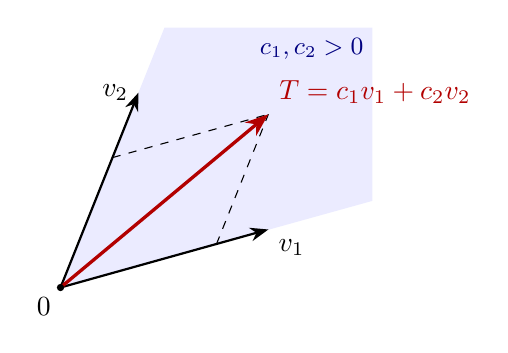
\begin{tikzpicture}[scale=1.1]
\fill[blue!8] (0,0)--(3.6,1.0)--(3.6,3.0)--(1.2,3.0)--cycle;
\draw[-{Stealth},thick] (0,0)--(2.4,0.67) node[below right]{$v_1$};
\draw[-{Stealth},thick] (0,0)--(0.9,2.25) node[left]{$v_2$};
\draw[dashed] (1.8,0.5)--(2.4,2.0);
\draw[dashed] (0.6,1.5)--(2.4,2.0);
\draw[-{Stealth},very thick,red!70!black] (0,0)--(2.4,2.0) node[above right]{$T=c_1v_1+c_2v_2$};
\fill (0,0) circle (1.2pt) node[below left]{$0$};
\node[blue!50!black] at (2.9,2.75) {\small $c_1,c_2>0$};
\end{tikzpicture}
\caption{The target stress must lie strictly inside the cone spanned by the two covariance directions (after Figure~4 of~\cite{OAI}). Strict interiority makes the representation stable under small perturbations of $v_1,v_2$.}
\label{fig:cone}
\end{figure}

\subsection{Sizes}
\paper{} (\S3.3) In the annulus the pulse amplitude and wavelength are
\[
A_{\rm wave}\asymp q^{-1/2-h/2},\qquad \ell_{\rm wave}\asymp q^{1/2+h/2},\qquad \frac{A_{\rm wave}}{q^{-1/2-h}}\asymp\frac{\ell_{\rm wave}}{q^{1/2}}\asymp q^{h/2}.
\]
\chk{} The averaged stress divergence is $A_{\rm wave}^2/\ell_r\asymp q^{-1-h}/q^{1/2}=q^{-3/2-h}$. This equals the size of $\partial_tu_\theta\asymp u_\theta/\tau\asymp q^{-1/2-h}/q$, so the pulses are exactly strong enough to enter the leading tangential balance. The pulses are also \emph{weaker} than the background by the factor $q^{h/2}$, and their wavelength is \emph{shorter} than the core radius by the same factor. This scale separation is what makes averaging accurate.

\subsection{Toy model 2: where the pulses get their energy}
\paper{} (\S2.2, \S3.3) For the linearized dynamics $L_{u_B}(w,\pi)=0$,
\[
\frac{\dd}{\dd t}\frac12\int|w|^2=-\sum_{i,j}\int w_iw_j\,\partial_j(u_B)_i-\int|\nabla w|^2 .
\]
The first term exchanges energy with the background shear; the second dissipates it.

\heur{} A simplified model explains the centrifugal part of the amplification. Take a rotating background $u_\theta=V(r)$ and a short-wavelength axisymmetric disturbance with wavevector $k=(k_r,0,k_z)$, ignoring viscosity for the moment. The linearized radial and azimuthal equations, after the pressure projection, reduce to
\[
\ddot w_r=-\frac{k_z^2}{|k|^2}\,\kappa^2\,w_r,\qquad \kappa^2:=\frac{2V}{r}\Big(V'+\frac Vr\Big)=\frac1{r^3}\frac{\dd}{\dd r}\big(rV\big)^2 .
\]
When the angular momentum $|rV|$ \emph{decreases} outward, $\kappa^2<0$ and the disturbance grows exponentially. This is Rayleigh's criterion~\cite{Ray}. In words: a parcel with surplus swirl is flung outward, and it lands among slower-turning fluid, which increases its relative surplus. This is the mechanism described in \S2.2 of~\cite{OAI}. The core is designed (\S\ref{sec:geometry}) so that the angular velocity drops steeply across the annulus. Generalized criteria for non-axisymmetric disturbances and swirling jets are due to Leibovich--Stewartson and Billant--Gallaire~\cite{LS,BG05,BG13}, and the paper cites these as precedents.

\paragraph{Growth, then decay.} \paper{} (\S2.2, \S3.3, Lemma~7.4) The pulses have nonzero angular frequency, so differential rotation \emph{tilts} their phase fronts and the radial wavenumber $|k_r|$ grows. Two effects follow. The geometric factor $k_z^2/|k|^2$ shrinks, which weakens amplification, and the viscous damping rate $\nu|k|^2$ grows. With a suitable initial wavelength, amplification wins first and damping wins later. Each pulse therefore rises and falls inside a finite time window with exponentially small tails (\paper{} Figure~3(b), envelope $P(v)$ in eq.~(7.12)). The tails are cut off, and the cutoff errors vanish to every order at the singularity. An exponentially small external force seeds each pulse (\S2.2).

\subsection{Keeping pulses from interfering}
\paper{} (\S3.3, \S6, Lemma~6.1) Pulses are placed on successively finer spatial and temporal scales as $t\uparrow1$, in dyadic bands $q\asymp2^{-\ell}$. To keep distinct pulses whose slow supports overlap from interacting, each wave is built as a function of an \emph{auxiliary} variable $Y\in\T^2$, and distinct labels receive disjoint supports in $Y$. The physical field is obtained by evaluating at a fixed phase map $Y=Y(r,t)$. Products of distinct pulses then vanish pointwise. Velocities are produced as curls of vector potentials, $w=\nabla\times A_{\rm wave}$, so they are \emph{exactly} divergence-free, and all chain-rule terms from $Y(r,t)$ are kept.

%======================================================================
\section{Correcting to infinite order}\label{sec:cycle}
%======================================================================

After the pulses cancel the leading stress, \eqref{eq:increment} leaves several kinds of error: linear terms $L_{u_B}(w,\pi)$, angular harmonics of $w\otimes w$, $Y$-dependent means, curl and cutoff errors, and defects in the radial integrals.

\paragraph{Background corrections.} \paper{} (\S5, Proposition~5.5) Before the pulses are added, the axisymmetric background is itself corrected in powers $q^{2nh}$, $n=1,2,\dots$, using axial diffusion ($\ell_r^2/\ell_z^2=q^{2h}$) as the small parameter. The result is a smooth background $(u_B,p_B)$ with
\[
\Res(u_B,p_B)=-(\partial_r+2/r)T_{{\rm phys},\theta}\,e_\theta-(\partial_r+1/r)T_{{\rm phys},z}\,e_z+E_B,
\]
where $T_{\rm phys}$ is supported in the annulus with leading term $T$, and $E_B$ is \emph{flat}: it is $O(q^N)$ with all derivatives, for every $N$.

\paragraph{The correction cycle.} \paper{} (\S3.4, Proposition~9.6) At stage $j$ one adds a divergence-free $\delta u_j$ and a pressure $\delta p_j$, which changes the residual by $L_{u^{[j]}}(\delta u_j,\delta p_j)+\nabla\cdot(\delta u_j\otimes\delta u_j)$. Each cycle performs four operations:
\begin{enumerate}[itemsep=1pt]
\item solve inhomogeneous wave-amplitude equations for the nonzero angular modes (Proposition~9.1, Lemma~9.2);
\item add signed amplitude increments whose cross-covariance with the leading pulses corrects the averaged stress (Proposition~7.6);
\item correct the angular mean with zero $Y$-average by inverting a fast auxiliary-time derivative (eq.~(8.20));
\item solve five radial moment equations, keeping all corrections compactly supported (eq.~(8.25)).
\end{enumerate}
After every operation the pressure is reconstructed and the \emph{full} residual is recomputed, so new error terms are fed into the next stage.

\paragraph{Bookkeeping.} \paper{} (eqs.~(9.8), (9.18)) For derivatives of order $m$ the stage-$j$ residual is bounded by $q^{h\sigma_j-K_m}$ (up to logarithms), with $K_m$ independent of $j$ and
\[
\sigma_0=\tfrac15,\qquad\sigma_{j+1}=\sigma_j+\tfrac1{10},\qquad\sigma_j\to\infty .
\]
Each cycle gains a fixed power $q^{h/10}$.

\paragraph{Summation.} \paper{} (\S3.4, Proposition~9.9) The infinitely many corrections are summed with cutoffs that equal one near $q=0$ and have shrinking supports. The cutoffs are applied to vector potentials and pressures before taking curls, which preserves incompressibility. This is a Borel-type summation. The derivative loss $K_m$ does not depend on the stage, so the cutoffs can be chosen to make every differentiated tail flat. The sum is locally finite for $q>0$. It defines smooth $(u_{\rm loc},p_{\rm loc})$ for $t<1$ that satisfy the flatness estimate \eqref{eq:flat} and keep the leading velocity growth.

\begin{figure}[h]
\centering
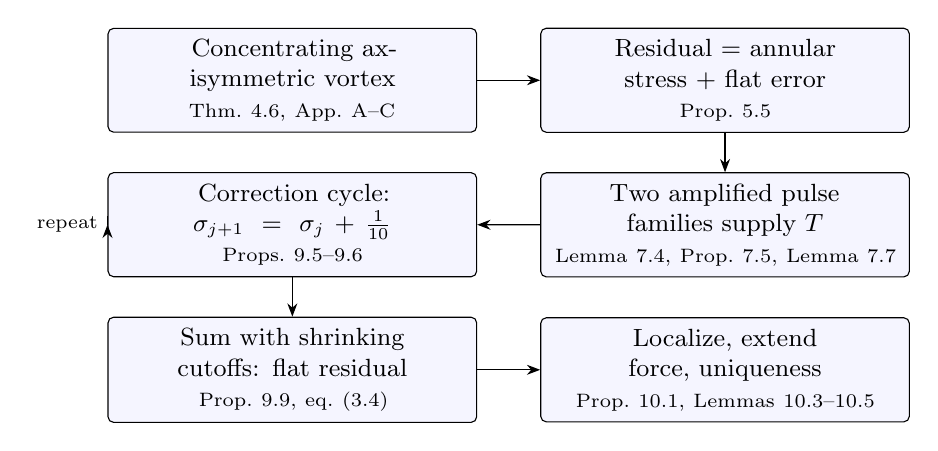
\begin{tikzpicture}[node distance=5mm,
 box/.style={draw,rounded corners=2pt,align=center,font=\small,text width=4.4cm,fill=blue!4,inner sep=4pt}]
\node[box] (a) {Concentrating axisymmetric vortex\\ \scriptsize Thm.~4.6, App.~A--C};
\node[box,right=8mm of a] (b) {Residual $=$ annular stress $+$ flat error\\ \scriptsize Prop.~5.5};
\node[box,below=of b] (c) {Two amplified pulse families supply $T$\\ \scriptsize Lemma~7.4, Prop.~7.5, Lemma~7.7};
\node[box,below=of a] (d) {Correction cycle: $\sigma_{j+1}=\sigma_j+\frac1{10}$\\ \scriptsize Props.~9.5--9.6};
\node[box,below=of d] (e) {Sum with shrinking cutoffs: flat residual\\ \scriptsize Prop.~9.9, eq.~(3.4)};
\node[box,right=8mm of e] (f) {Localize, extend force, uniqueness\\ \scriptsize Prop.~10.1, Lemmas~10.3--10.5};
\draw[-{Stealth}] (a)--(b); \draw[-{Stealth}] (b)--(c); \draw[-{Stealth}] (c)--(d); \draw[-{Stealth}] (d)--(e); \draw[-{Stealth}] (e)--(f);
\draw[-{Stealth}] (d.west) to[out=200,in=160,looseness=4] node[left,font=\scriptsize]{repeat} (d.west);
\end{tikzpicture}
\caption{Architecture of the proof (compare Figures~5--6 of~\cite{OAI}).}
\end{figure}

%======================================================================
\section{Finishing: localization, the force, energy and uniqueness}\label{sec:finish}
%======================================================================

\subsection{Localization}
\paper{} (\S3.5, Proposition~10.1) The local field is written as $u_{\rm loc}=\curl A+Be_\theta$ (Theorem~3.1(i)). One multiplies $A$, $B$ and $p_{\rm loc}$ by $c=\chi_x\chi_t$, where $\chi_x$ is compactly supported and axisymmetric, $\chi_t$ vanishes for small $t$, and both equal one near $(0,1)$. One then takes the curl \emph{after} multiplying:
\[
u=\curl(cA)+cBe_\theta=c\,u_{\rm loc}+\nabla c\times A .
\]
This field is exactly divergence-free, has fixed compact support, and agrees with the local field near the singular point. The extra force created by the cutoff lives where $c$ varies. Near $t=1$ that is away from the origin, where the heat exterior and Theorem~3.1(ii) give smooth limits.

\subsection{Extending the force past the singular time}
\paper{} (Lemmas~10.2--10.3) Every derivative of $f=\Res(u,p)$ has a limit as $t\uparrow1$, uniformly in $x$. A Borel-lemma construction,
\[
f(x,1+\sigma)=\sum_{j\ge0}\chi_0(b_j\sigma)\frac{\sigma^j}{j!}F_j(x),
\]
with $F_j$ the limiting $j$-th time derivatives and integers $b_j$ growing fast enough, extends $f$ smoothly to $t>1$ with support in $K\times[0,2]$. \heur{} After $t=1$ no smooth solution exists. The extension is needed only because (C) asks for a force defined for all $t\ge0$.

\subsection{Energy}\label{sec:energy}
\paper{} (Lemma~10.4) With $F(t)=\int_0^t\|f(s)\|_{L^2}\dd s$,
\[
\|u(t)\|_{L^2}^2+2\int_0^t\|\nabla u(s)\|_{L^2}^2\dd s\le F(t)^2,\qquad 0\le t<1 .
\]
\chk{} Pairing \eqref{eq:NS} with $u$ (with compact support, the transport and pressure terms integrate to zero) gives $\tfrac12\frac{\dd}{\dd t}\|u\|^2+\|\nabla u\|^2=\avg{f,u}\le\|f\|\|u\|$. Hence $\frac{\dd}{\dd t}\|u\|\le\|f\|$ and $\|u(t)\|\le F(t)$. Integrating once more gives the stated bound. Since $f$ is compactly supported and smooth, $F(1)<\infty$.

\subsection{Why no global solution exists}
\paper{} (Lemma~10.5) Fix $T<1$. Any smooth solution $(v,P)$ on $[0,T]$ with the same force, zero data and $v\in L^\infty_tL^2_x$ equals $u$. The proof compares $w=v-u$ on expanding balls. The delicate point is the pressure, because no growth condition is imposed on $P$. The pressure gradient is recovered from the equation as $\nabla\pi^*$ with $\pi^*=\sum_{i,j}R_iR_jg_{ij}$ (Riesz transforms), and the boundary pressure flux is then absorbed by the dissipation. A hypothetical global smooth bounded-energy solution would agree with $u$ on every $[0,T]$, so it would be unbounded near $(0,1)$. This contradiction proves Theorem~\ref{thm:main}.

\subsection{Viscosity and the torus}\label{sec:torus}
\paper{} (\S3, Corollary~10.6) \chk{} If $(u,p,f)$ works at $\nu=1$, then $u_\nu(x,t)=\sqrt\nu\,u(x/\sqrt\nu,t)$, $p_\nu=\nu p(x/\sqrt\nu,t)$, $f_\nu=\sqrt\nu f(x/\sqrt\nu,t)$ works at viscosity $\nu$, with the same singular time. Indeed every term of the equation picks up the same factor $\sqrt\nu$. For the torus, one shrinks the compact solution with $\tilde u(x,t)=\lambda u(\lambda x,\lambda^2(t-t_0))$ ($t_0=1-\lambda^{-2}$) until it fits inside one periodic cell, then periodizes:
\[
U(x,t)=\sum_{k\in\mathbb Z^3}\tilde u(x+k,t).
\]
Distinct translates have disjoint supports, so the nonlinearity does not mix them and $U$ solves the periodic equations exactly. Uniqueness on the torus is a direct Gronwall argument. This gives alternative~(D).

%======================================================================
\section{What the Lean formalization certifies}\label{sec:lean}
%======================================================================

\paper{} (Repository~\cite{OAILean}, commit \texttt{f9e8bc5b38b6e212696e8a30e3e91517af887bbd}) The repository uses Lean \texttt{v4.34.0-rc2} with Mathlib. Its \texttt{NavierStokes/} directory contains 817 Lean files, about 22.8\,MB of source; we counted these from the Git tree at that commit.

\paragraph{The statement.} The target statements are in \texttt{ComparatorChallenges/NavierStokes.lean}. This file is a standalone adaptation of Google DeepMind's \emph{Formal Conjectures} formalization of Fefferman's problem~\cite{FC}, and it imports only Mathlib. It defines:
\begin{itemize}[itemsep=1pt]
\item \texttt{InitialVelocityConditionDecay}: $u^\circ$ is smooth, divergence-free, and $\|D^mu^\circ(x)\|\le C/(1+\|x\|)^K$ for all $m,K$;
\item \texttt{ForceConditionDecay}: $f$ is smooth on $\R^3\times[0,\infty)$ and $\|D^m_{x,t}f\|\le C/(1+\|x\|+t)^K$;
\item \texttt{NavierStokesExistenceAndSmoothnessRn}: the PDE holds for all $x$ and $t\ge0$, with the time derivative taken within $[0,\infty)$; plus incompressibility, the initial condition, $C^\infty$ velocity and pressure on $\R^3\times[0,\infty)$, $v(\cdot,t)\in L^2$, and a uniform energy bound;
\item periodic analogues, which require periodic velocity and pressure (following the Clay errata).
\end{itemize}
The two theorems are
\begin{center}\small
\texttt{navier\_stokes\_breakdown\_R3 (nu) (hnu : nu > 0) :}\\
\texttt{\ \ $\exists$ u0 f, InitialVelocityConditionDecay u0 $\wedge$ ForceConditionDecay f $\wedge$}\\
\texttt{\ \ \ \ $\neg\,\exists$ v p, NavierStokesExistenceAndSmoothnessRn nu u0 f v p}
\end{center}
and its periodic counterpart \texttt{navier\_stokes\_breakdown\_periodic}. In the challenge file both are stated with \texttt{sorry}; the repository supplies the proofs.

\paragraph{The check.} The Comparator configuration (\texttt{ComparatorChallenges/NavierStokes.json}) names the solution module \texttt{NavierStokes.ComparatorSolution}, enables the independent \texttt{nanoda} kernel, and permits only \texttt{propext}, \texttt{Quot.sound} and \texttt{Classical.choice}. Comparator~\cite{Comparator} checks that the proved theorems have exactly the challenge statements and that nothing beyond those axioms is used. The bridge files \texttt{NavierStokes/ComparatorR3Theorem.lean} and \texttt{ComparatorTheorem.lean} derive these statements from the formal versions of Theorem~1.1 and Corollary~10.6, including the decay bounds for the rescaled force and the zero initial datum.

\begin{statusbox}{What this note did and did not verify}
We read the statements, the bridge files and the Comparator configuration at the pinned commit. We did \emph{not} build the project, replay the kernel check or run Comparator. The Justin Sun Prize catalog entry for JSP-000005 likewise notes that independent review remains pending. Formal verification certifies that \emph{the stated theorem} follows from Mathlib's foundations. Whether the Lean statement faithfully encodes Fefferman's problem is a separate, human question. The definitions above are short enough for a reader to check that they match the Clay text.
\end{statusbox}

%======================================================================
\section{Assessment and open directions}
%======================================================================

\begin{itemize}[itemsep=2pt]
\item \textbf{What is new.} The flow is honestly viscous: radial diffusion stays in the leading balance throughout. The force is $C^\infty$ and compactly supported in space and time. The cancellation that makes the force smooth is carried out to \emph{infinite} order. Earlier forced constructions either worked for Euler or hypodissipative models, or used forces of limited regularity~\cite{CMZ,CMZZ,ABC}.
\item \textbf{The role of the force.} The force is not a perturbation: it is the residual of a designed flow, and it is large in the cutoff region. The result shows that the class of smooth forces allowed by (C) is rich enough to drive singularities. It says nothing direct about unforced fluids.
\item \textbf{Toward (A)/(B).} An unforced blowup would require a vortex that sustains its own annular momentum flux, with no external seeding of the pulses and no residual to absorb. Whether self-generated instabilities around a collapsing anisotropic vortex could do this is, as far as we know, entirely open. Tao's averaged-equation result~\cite{Tao} remains the main evidence that energy methods alone cannot settle the question.
\item \textbf{Verification.} The decisive next steps are independent mathematical review of the 166 pages, an independent build and Comparator run of the Lean development, and human review of the formal statement against~\cite{Fef}.
\end{itemize}

%======================================================================
\appendix
\section{A reading map of the paper}
%======================================================================

\begin{center}\small
\begin{tabularx}{\linewidth}{@{}l l X@{}}
\toprule
\S & Pages & Content and key results\\
\midrule
1--2 & 1--6 & Theorem~1.1; history; physical description (core, annulus and pulses, exterior).\\
3 & 6--24 & Full proof outline; Theorem~3.1 (local construction with flat residual); notation and averaging conventions; Figures~5--6.\\
4 & 24--44 & Leading profiles in similarity variables; stress from radial integration (Proposition~4.2); five radial integrals and joining (Lemma~4.4); admissible stress cone (Lemma~4.5); Theorem~4.6.\\
5 & 45--61 & Background corrections in powers $q^{2nh}$; flat remainder; Proposition~5.5.\\
6 & 62--72 & Auxiliary torus $Y\in\T^2$, dyadic bands, separation of oscillatory supports (Lemma~6.1).\\
7 & 73--87 & Phases, amplitude equations and growth/decay envelope (Lemmas~7.1, 7.4); stress realization (Propositions~7.5--7.6); curl corrections (Lemma~7.7, Corollary~7.8).\\
8 & 88--99 & Compactly supported mean corrections; inverting the fast auxiliary derivative; radial moment equations.\\
9 & 100--115 & Residual improvement cycle (Propositions~9.5--9.6), summation (Proposition~9.9).\\
10 & 116--125 & Localization (Proposition~10.1); force extension (Lemma~10.3); energy (Lemma~10.4); uniqueness (Lemma~10.5); torus (Corollary~10.6).\\
A & 126--143 & Radial moments and the exact heat exterior (Lemma~A.6, Proposition~A.7).\\
B & 144--156 & Analytic profiles near the axis (Proposition~B.2) and their continuation.\\
C & 157--164 & Realizing the admissible stress cone (Propositions~C.2--C.3).\\
\bottomrule
\end{tabularx}
\end{center}
\noindent Suggested route for a first reading: \S2, then \S3.1--3.5 with Figures~5--6, then Lemma~10.5 and Corollary~10.6, then \S7 for the pulse mechanism.

\section{Glossary of notation}
\begin{center}\small
\begin{tabularx}{\linewidth}{@{}l X@{}}
\toprule
$\tau=1-t$ & time to the singularity.\\
$h\in(0,1/100)$; $A=\tfrac12+h$, $D=\tfrac12-h$ & anisotropy exponent; velocity and axial-length exponents.\\
$q$; $(X,\eta)$ & concentration scale ($q\asymp\tau+|z|^{1/D}$); similarity coordinates, $X=r^2/2q$, $z=q^D\eta$.\\
$E,U,\Pi,V_0$ & azimuthal, axial and pressure profiles; $ru_r^{(0)}$.\\
$X_a<X<X_b$ & the pulse annulus; $X\ge X_{\rm ext}$: heat exterior.\\
$T=(T_{r\theta},T_{rz})$ & annular stress: radial fluxes of azimuthal and axial momentum.\\
$v_1,v_2$; $c_1,c_2$ & covariance directions of the two pulse families; their positive weights.\\
$\Res(u,p)$ & momentum residual \eqref{eq:residual}; the force is $f=\Res(u,p)$.\\
flat & bounded by $q^N$ for every $N$, with all derivatives.\\
$Y\in\T^2$; $\avg{\cdot}$ & auxiliary oscillation variable; the angular and auxiliary average (eq.~(3.8)).\\
$\sigma_j$ & residual decay exponent after $j$ correction cycles.\\
\bottomrule
\end{tabularx}
\end{center}

\section*{Originality and attribution}
All mathematical results described here are due to the authors of~\cite{OAI} and of the works cited. The Lean formalization is due to~\cite{OAILean}, and the formal problem statement is adapted from~\cite{FC}. This note contributes only exposition: the organization, the explanations, the scale checks marked \chk{} (Table~\ref{tab:scales}, the energy and viscosity-scaling computations), the two toy models marked \heur{}, the reading map and the glossary. Section and equation numbers refer to the PDF at~\cite{OAI} as downloaded on 29 October 2026.

\begin{thebibliography}{99}\small
\bibitem{OAI} OpenAI, \emph{Finite time blowup for Navier--Stokes}, preprint, September 2026, 166~pp. \url{https://cdn.openai.com/pdf/32d9f210-8b73-45e0-91bc-82a30aef8a9a/navier-stokes.pdf}
\bibitem{OAILean} OpenAI, \emph{NavierStokesAndEuler} (Lean~4 formalization), commit \texttt{f9e8bc5b38b6e212696e8a30e3e91517af887bbd}. \url{https://github.com/openai/NavierStokesAndEuler}
\bibitem{Fef} C.~L. Fefferman, \emph{Existence and smoothness of the Navier--Stokes equation}, Clay Mathematics Institute Millennium Problem statement. \url{https://www.claymath.org/wp-content/uploads/2022/06/navierstokes.pdf}
\bibitem{FC} Google DeepMind, \emph{Formal Conjectures}, \texttt{FormalConjectures/Millenium/NavierStokes.lean}, commit \texttt{8bf45ed7}. \url{https://github.com/google-deepmind/formal-conjectures}
\bibitem{Comparator} Lean FRO, \emph{Comparator}. \url{https://github.com/leanprover/comparator}
\bibitem{Leray} J.~Leray, Sur le mouvement d'un liquide visqueux emplissant l'espace, \emph{Acta Math.} 63 (1934), 193--248.
\bibitem{CKN} L.~Caffarelli, R.~Kohn, L.~Nirenberg, Partial regularity of suitable weak solutions of the Navier--Stokes equations, \emph{Comm. Pure Appl. Math.} 35 (1982), 771--831.
\bibitem{ESS} L.~Escauriaza, G.~A.~Seregin, V.~\v{S}ver\'ak, $L_{3,\infty}$-solutions of the Navier--Stokes equations and backward uniqueness, \emph{Russian Math. Surveys} 58 (2003), 211--250.
\bibitem{NRS} J.~Ne\v{c}as, M.~R\r{u}\v{z}i\v{c}ka, V.~\v{S}ver\'ak, On Leray's self-similar solutions of the Navier--Stokes equations, \emph{Acta Math.} 176 (1996), 283--294.
\bibitem{Tsai} T.-P.~Tsai, On Leray's self-similar solutions of the Navier--Stokes equations satisfying local energy estimates, \emph{Arch. Ration. Mech. Anal.} 143 (1998).
\bibitem{Tao} T.~Tao, Finite time blowup for an averaged three-dimensional Navier--Stokes equation, \emph{J. Amer. Math. Soc.} 29 (2016), 601--674.
\bibitem{BV} T.~Buckmaster, V.~Vicol, Nonuniqueness of weak solutions to the Navier--Stokes equation, \emph{Ann. of Math.} 189 (2019), 101--144.
\bibitem{ABC} D.~Albritton, E.~Brué, M.~Colombo, Non-uniqueness of Leray solutions of the forced Navier--Stokes equations, \emph{Ann. of Math.} 196 (2022), 415--455.
\bibitem{CMZ} D.~Córdoba, L.~Martínez-Zoroa, Blow-up for the incompressible 3D-Euler equations with uniform $C^{1,\frac12-\epsilon}\cap L^2$ force, arXiv:2309.08495 (2023).
\bibitem{CMZZ} D.~Córdoba, L.~Martínez-Zoroa, F.~Zheng, Finite time blow-up for the hypodissipative Navier--Stokes equations with a force in $L^1_tC^{1,\epsilon}_x\cap L^\infty_tL^2_x$, \emph{Arch. Ration. Mech. Anal.} 250 (2026), 38.
\bibitem{CC} A.~D.~D.~Craik, W.~O.~Criminale, Evolution of wavelike disturbances in shear flows: a class of exact solutions of the Navier--Stokes equations, \emph{Proc. R. Soc. Lond. A} 406 (1986), 13--26.
\bibitem{Ray} Lord Rayleigh, On the dynamics of revolving fluids, \emph{Proc. R. Soc. Lond. A} 93 (1917), 148--154.
\bibitem{LS} S.~Leibovich, K.~Stewartson, A sufficient condition for the instability of columnar vortices, \emph{J. Fluid Mech.} 126 (1983), 335--356.
\bibitem{BG05} P.~Billant, F.~Gallaire, Generalized Rayleigh criterion for non-axisymmetric centrifugal instabilities, \emph{J. Fluid Mech.} 542 (2005), 365--379.
\bibitem{BG13} P.~Billant, F.~Gallaire, A unified criterion for the centrifugal instabilities of vortices and swirling jets, \emph{J. Fluid Mech.} 734 (2013), 5--35.
\end{thebibliography}

\end{document}
